\documentclass[a4paper, 12pt, final, garamond]{book}
\usepackage{cours-preambule}

\raggedbottom

\makeatletter
\renewcommand{\@chapapp}{M\'ecanique -- chapitre}
\makeatother

% \toggletrue{student}
% \HideSolutionstrue
\toggletrue{corrige}
\renewcommand{\mycol}{black}
% \renewcommand{\mycol}{gray}

\begin{document}
\setcounter{chapter}{3}

\chapter{\cswitch{Correction du TD d'application}{TD application~: approche
	  \'energ\'etique}}

\resetQ
\section{Intérêt des raisonnements énergétiques}
\QR{%
	On lance une balle avec une vitesse initiale $v_0$ vers le haut depuis
	l'altitude $z = 0$. Déterminer la hauteur maximale atteinte par la balle
	en négligeant tout frottement.
}{%
	\begin{minipage}[t]{0.48\linewidth}
		À $t=0$, la balle est lancée en $z = 0$ avec une vitesse $\vfo =
			v_O\uz$. Elle va monter en altitude en perdant de l'énergie cinétique et
		en gagnant en énergie potentielle. \bigbreak
		Le système \{masse\} n'est soumis qu'au poids, qui est conservatif~; le
		système est donc conservatif et l'énergie mécanique se conserve~:
	\end{minipage}
	\hfill
	\begin{minipage}[t]{0.50\linewidth}
		~
		\begin{center}
			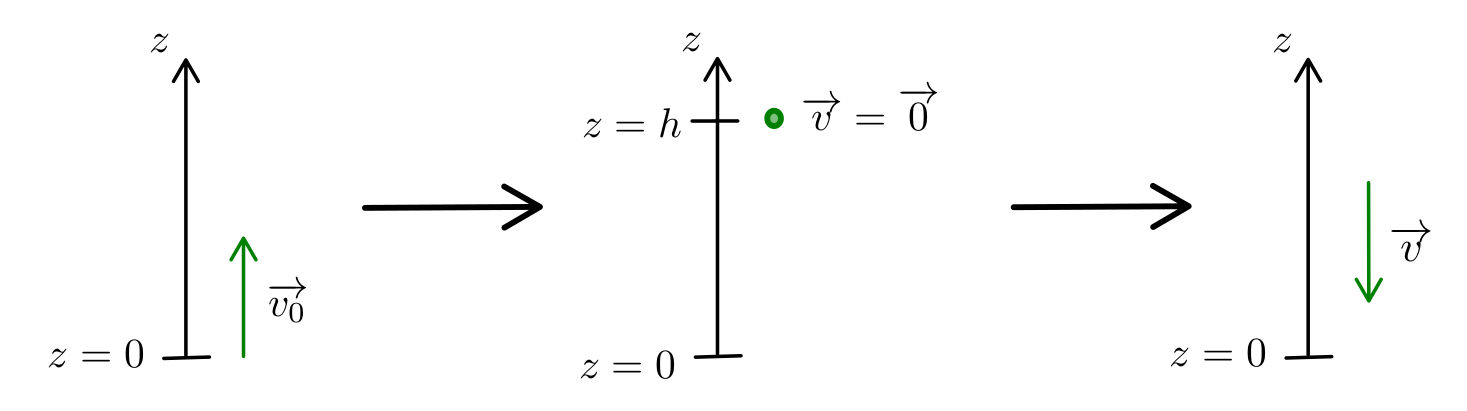
\includegraphics[width=\linewidth]{hmax_vert_corr}
			\captionof{figure}{Schéma de la situation}
			\label{fig:penduleztt}
		\end{center}
	\end{minipage} \bigbreak
	\[\dv{\Ec_m}{t} = 0\]
	Ainsi,\vspace*{-24pt}
	\begin{align*}
		\Ec_m(0)  & = \Ec_m(t_{\max})
		\\\Lra
		\frac{1}{2}\cancel{m}v_0{}^2 + \underbracket{mgz_0}_{=0}
		          & =
		\frac{1}{2}\cancel{m}v(t_{\max})^2 + \cancel{m}gh
		\\\Lra
		\Aboxed{h & = \sqrt{\frac{v_0{}^2}{2g}}}
		\qed
	\end{align*}
}
\QR{%
On considère un pendule simple (masse $m$ ponctuelle, longueur $\ell$,
pas de frottements). On fait partir ce pendule de la verticale ($\tt =
	0$, en bas) en lui communiquant une vitesse initiale $v_0$. Déterminer
l'expression de l'amplitude maximale $\tt_{\max}$ du mouvement.
}{%
\begin{minipage}[t]{0.70\linewidth}
	Le système est conservatif puisque le poids est une force conservative
	et que le travail de la force de tension est nul ($\Tf \perp \vf$). On
	peut donc utiliser le TEM en déterminant l'énergie potentielle en
	fonction de $\tt$. \bigbreak
	On prend la référence d'altitude $z = 0$ en bas du pendule. La longueur
	du pendule étant $\ell$, on trouve l'altitude en projetant le point M
	sur l'axe $z$ pour trouver
\end{minipage}
\hfill
\begin{minipage}[t]{0.28\linewidth}
	\vspace*{-1cm}
	\begin{center}
		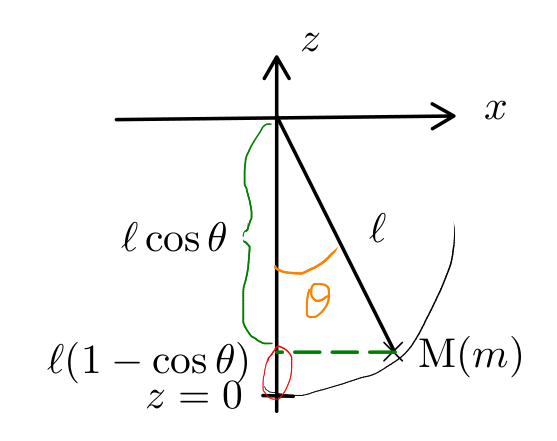
\includegraphics[width=\linewidth]{thetamax_pend_corr}
		\captionsetup{justification=centering}
		\captionof{figure}{Schéma pour $z(\tt)$}
		\label{fig:penduleztt}
	\end{center}
\end{minipage}
\[z(\tt) = \ell(1-\cos\tt)\]
Ainsi,
\begin{align*}
	\D_{\ABr}\Ec_m         & =0
	\\\Lra
	\frac{1}{2}\cancel{m}v_0{}^2 + \underbracket{mgz_0}_{=0}
	                       & =
	\frac{1}{2}\cancel{m}v_{\max}{}^2 + \cancel{m}gz_{\max}
	\\\Lra
	\ell(1-\cos\tt_{\max}) & = \frac{v_0{}^2}{2g}
	\\\Lra
	\Aboxed{\cos\tt_{\max} & = 1 - \frac{v_0{}^2}{2g\ell}}
	\qed
\end{align*}
Cette équation est valable si $v_0{}^2/2g\ell < 2$, sinon
$\cos\tt_{\max} < -1$. Cette condition traduit le fait que le pendule ne
fait pas des tours, i.e. ne dépasse pas $\tt = \pi$.
}

\resetQ
\section{Curling}
\enonce{%
	Le curling est un sport de précision pratiqué sur la glace avec des pierres en
	granite, taillées et polies selon un gabarit international. Le but est de placer
	les pierres le plus près possible d'une cible circulaire dessinée sur la glace,
	appelée la maison.
	\smallbreak
	\noindent
	\begin{minipage}{0.60\linewidth}
		Nous envisageons le lancer d'une pierre assimilée à un point M de masse $m =
			\SI{20}{kg}$ glissant selon l'axe O$x$ vers le point M$_0$ visé (la maison).
		La pierre est lancée de la position initiale O avec une vitesse $\vfo =
			v_0\ux$, la maison se trouvant à la distance $D = {\rm OM_0} = \SI{25}{m}$
		du point O.
	\end{minipage}
	\hfill
	\begin{minipage}{0.35\linewidth}
		\begin{center}
			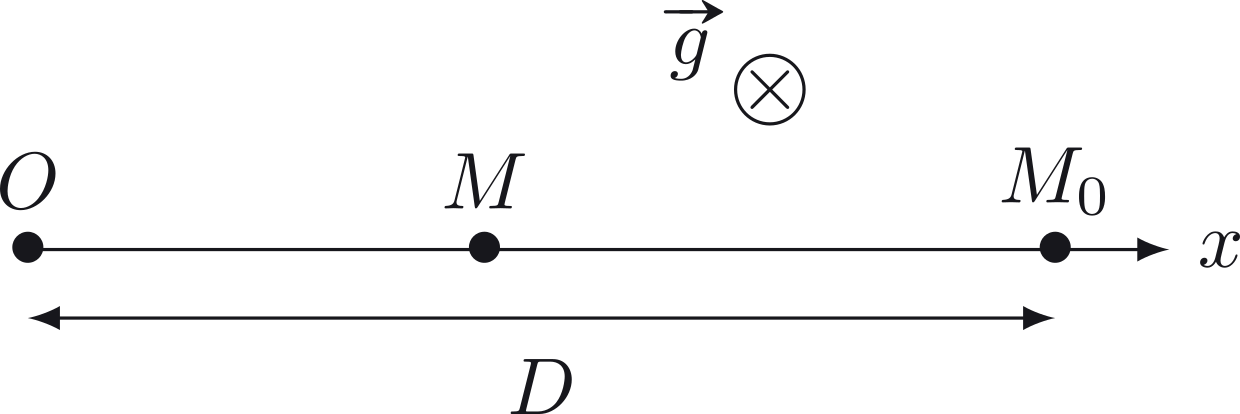
\includegraphics[width=\linewidth]{curling_plain}
		\end{center}
	\end{minipage}
	\bigbreak
	Nous supposerons que la force de frottement solide $\Ff = -F_0\ux$ de la glace
	sur la pierre est constante pendant toute la glissade et s'annule lorsque la
	vitesse de la pierre s'annule. Nous prendrons $F_0 = \SI{3.0}{N}$. Nous
	négligerons par ailleurs toute force de frottement fluide.
	\smallbreak
	Le lancer étudié est supposé gagnant~: la pierre atteint la maison et s'y
	arrête.
}

\QR{%
Que valent les énergies cinétiques initiale $\Ec_{c,I}$ et finale
$\Ec_{c,F}$ de la pierre ?
}{%
On a simplement
\[
	\Ec_{c,I} = \frac{1}{2}mv_0{}^2
	\qet
	\Ec_{c,F} = 0
\]
}
\QR{%
	Calculer le travail des forces appliquées sur la pierre pendant la
	glissade.
}{%
	\begin{minipage}[t]{0.40\linewidth}
		\begin{itemize}[label=$\diamond$, leftmargin=10pt]
			\bitem{Système~:} \{pierre\}
			\bitem{Référentiel~:} $\Rc\ind{piste}$, galiléen
			\bitem{Repère~:} $(\Or,\ux,\uz)$
			\bitem{Repérage~:}
			\begin{gather*}
				\OM = x\ux\\
				\vv{\rm OM_0} = D\ux\\
				\vf = \xp\ux
			\end{gather*}
		\end{itemize}
	\end{minipage}
	\hfill
	\begin{minipage}[t]{0.65\linewidth}
		~
		\begin{center}
			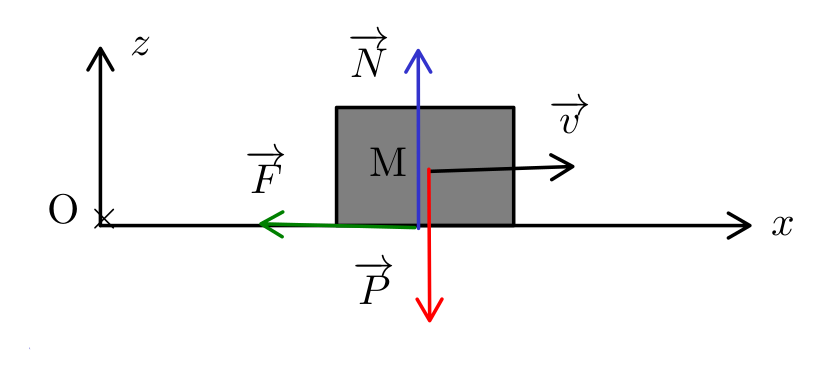
\includegraphics[width=.8\linewidth]{curling_corr}
			\captionof{figure}{Schéma de la situation}
			\label{fig:curling}
		\end{center}
	\end{minipage} \bigbreak
	\begin{itemize}[label=$\diamond$, leftmargin=10pt]
		\bitem{BDF et BDW~:}
		\[
			\begin{array}{ll}
				\textbf{Poids}       & \Pf = -mg\uz  \\
				\textbf{Réaction}    & \Nf = N\uz    \\
				\textbf{Frottements} & \Ff = -F_0\ux
			\end{array}
			\quad\Ra\quad
			\begin{array}{llll}
				W_{\rm OM_0}(\Pf)                      & = \Pf\cdot\vv{\rm OM_0} & =
				-mgD(\underbracket{\uz\cdot\ux}_{=0})  & = 0                         \\
				W_{\rm OM_0}(\Nf)                      & = \Nf\cdot\vv{\rm OM_0} & =
				ND(\underbracket{\uz\cdot\ux}_{=0})    & = 0                         \\
				W_{\rm OM_0}(\Ff)                      & = \Ff\cdot\vv{\rm OM_0} & =
				-F_0D(\underbracket{\ux\cdot\ux}_{=1}) & = -F_0D
			\end{array}
		\]
	\end{itemize}
}
\QR{%
	Appliquer le théorème de l'énergie cinétique à la pierre et en déduire
	la vitesse initiale $v_0$.
}{%
	Ici,\vspace*{-24pt}
	\begin{align*}
		\D_{\rm OM_0}\Ec_c      & = \sum_i W_{\rm OM_0}(\Ff_i)
		\\\Lra
		0 - \frac{1}{2}mv_0{}^2 & = -F_0D
		\\\Lra
		\Aboxed{v_0             & = \sqrt{\frac{2F_0D}{m}}}
		\qed
		\qavec
		\left\{
		\begin{array}{rcl}
			F_0 & = & \SI{3.0}{N} \\
			D   & = & \SI{25}{m}  \\
			m   & = & \SI{20}{kg}
		\end{array}
		\right.                                                \\
		\AN
		\Aboxed{v_0             & = \SI{2.7}{m.s^{-1}}}
	\end{align*}
}

\resetQ
\section{Piégeage d'un électron}
\enonce{%
	Considérons le mouvement selon un axe (O$z$) d'un électron de masse $m =
		\SI{9.1e-31}{kg}$ et de charge $-e = \SI{-1.6e-19}{C}$ dans un dispositif de
	piégeage. Il est soumis uniquement à des forces conservatives, d'énergie
	potentielle totale $\Ec_p(z)$ telle que~:
	\[\Ec_p(z) = \frac{eV_0}{2d^2}z^2\]
	avec $V_0 = \SI{5.0}{V}$ et $d = \SI{6.0}{mm}$.
}

\QR{%
	Tracer l'allure de $\Ec_p(z)$. Identifier la position d'équilibre et
	donner sa stabilité.
}{%
	\begin{minipage}[t]{0.30\linewidth}
		~
		\begin{center}
			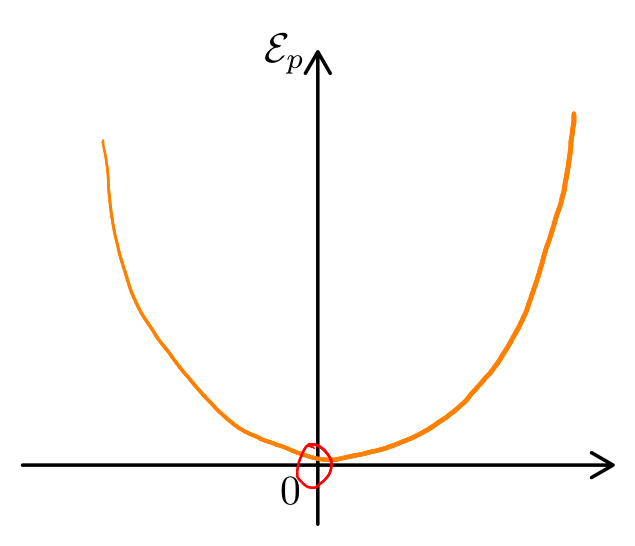
\includegraphics[width=\linewidth]{piege_elec_corr}
			\captionof{figure}{$\Ec_p(z)$}
			\label{fig:piegeelec}
		\end{center}
	\end{minipage}
	\hfill
	\begin{minipage}[t]{0.65\linewidth}
		On trace l'énergie potentielle, qui est \textbf{évidemment} une
		parabole convexe. On trouve le point d'équilibre en calculant sa
		dérivée et en trouvant quand elle s'annule~; visuellement, la
		dérivée s'annule en $z\ind{eq} = 0$, mathématiquement
		\[\eval{\dv{\Ec_p}{z}}_{z\ind{eq}} = \frac{eV_0}{d^2}z\ind{eq} = 0 \Lra
			\boxed{z\ind{eq} = 0}\]
		On trouve sa stabilité en évaluant sa dérivée seconde en ce point,
		et il sera stable si elle est positive. En tant que fonction convexe
		en ce point, il est visiblement stable. On calcule~:
	\end{minipage}
	\[\boxed{\eval{\dv[2]{\Ec_p}{z}}_{z\ind{eq}} = \frac{eV_0}{d^2} > 0}\]
	Il est donc bien stable.
}
\QR{%
Calculer la fréquence des oscillations de l'électron dans le piège.
}{%
Tout système conservatif autour de son point d'équilibre stable est
régit par une équation d'oscillateur harmonique, faisant donc apparaître
la pulsation propre $\w_0$. Il suffit pour démontrer cela d'utiliser la
caractéristique principale d'un système conservatif~: le fait que son
énergie mécanique se conserve, i.e. $\dv{\Ec_m}{t} = 0$. En effet, le
TPC nous indique
\[\dv{\Ec_m}{t} = \sum_i \underbracket[1pt][.8em]{\Pc(\Ff_{{\rm
				NC},i})}_{\mathclap{=0\text{ car conservatif}}} = 0\]
On nous donne $\Ec_p(z)$, donc pour avoir $\Ec_m$ il faut trouver la
vitesse de la particule. Rien n'est indiqué dans l'énoncé, mais le
problème n'indique qu'un potentiel selon $\uz$~; on peut supposer que la
vitesse ne se fait que selon $\uz$ également, et qu'on a donc $\vf =
	\zp\uz$. Ainsi,
\begin{align*}
	\dv{\Ec_m}{t}                                     & = 0
	\\\Lra
	\dv{t}(\Ec_c + \Ec_p)                             & = 0
	\\\Lra
	\dv{t}(\frac{1}{2}m\zp^2 + \frac{eV_0}{2d^2}z^2)  & = 0
	\\\Lra
	m\cancel{\zp}\zpp + \frac{eV_0}{d^2}z\cancel{\zp} & = 0
	\\\Lra
	\Aboxed{\zpp + \w_0{}^2z                          & = 0}
	\qavec
	\boxed{\w_0 = \sqrt{\frac{eV_0}{md^2}}}
\end{align*}
Étant donné que $\w_0 = 2\pi f_0$, on obtient finalement
\begin{align*}
	\Aboxed{f_0 & = \frac{1}{2\pi}\sqrt{\frac{eV_0}{md^2}}}
	\qed
	\qavec
	\left\{
	\begin{array}{rcl}
		e   & = & \SI{1.6e-19}{C}  \\
		V_0 & = & \SI{5.0}{V}      \\
		m   & = & \SI{9.1e-31}{kg} \\
		d   & = & \SI{6.0e-3}{m}
	\end{array}
	\right.                                                 \\
	\AN
	\Aboxed{f_0 & = \SI{25}{MHz}}
\end{align*}
}
\QR{%
	Exprimer la résultante des forces $\Ff$ sur l'électron. On rappelle
	qu'en coordonnées cartésiennes, on a
	\[\gd{f}(x,y,z) = \pdv{f}{x}\ux + \pdv{f}{y}\uy + \pdv{f}{z}\uz \]
}{%
	Une force conservative dérive d'une énergie potentielle selon
	\begin{align*}
		\Ff         & = -\gd\Ec_p
		\\\Lra
		\Ff         & =
		-\mqty(\DS\pdv{\Ec_p}{x}                \\[1em]\DS\pdv{\Ec_p}{y}\\[1em]\DS\pdv{\Ec_p}{z})
		=
		-\mqty(0                                \\0\\\DS\frac{eV_0}{d^2}z)
		\\\Lra
		\Aboxed{\Ff & = - \frac{eV_0}{d^2}z\uz}
		\qed
	\end{align*}
}

\resetQ
\section{Balle dans un tonneau}
\enonce{%
	\begin{minipage}{0.60\linewidth}
		Une balle, assimilée à un point matériel M de masse $m$, est lâchée sur une
		rampe sans vitesse initiale depuis le point A d'une hauteur $h$ par rapport
		au point O le bout de la rampe. Elle achève sa course dans un tonneau
		circulaire de rayon $R$ lui permettant éventuellement de faire des
		\textit{loopings}. On néglige les frottements.
	\end{minipage}
	\hfill
	\begin{minipage}{0.35\linewidth}
		\begin{center}
			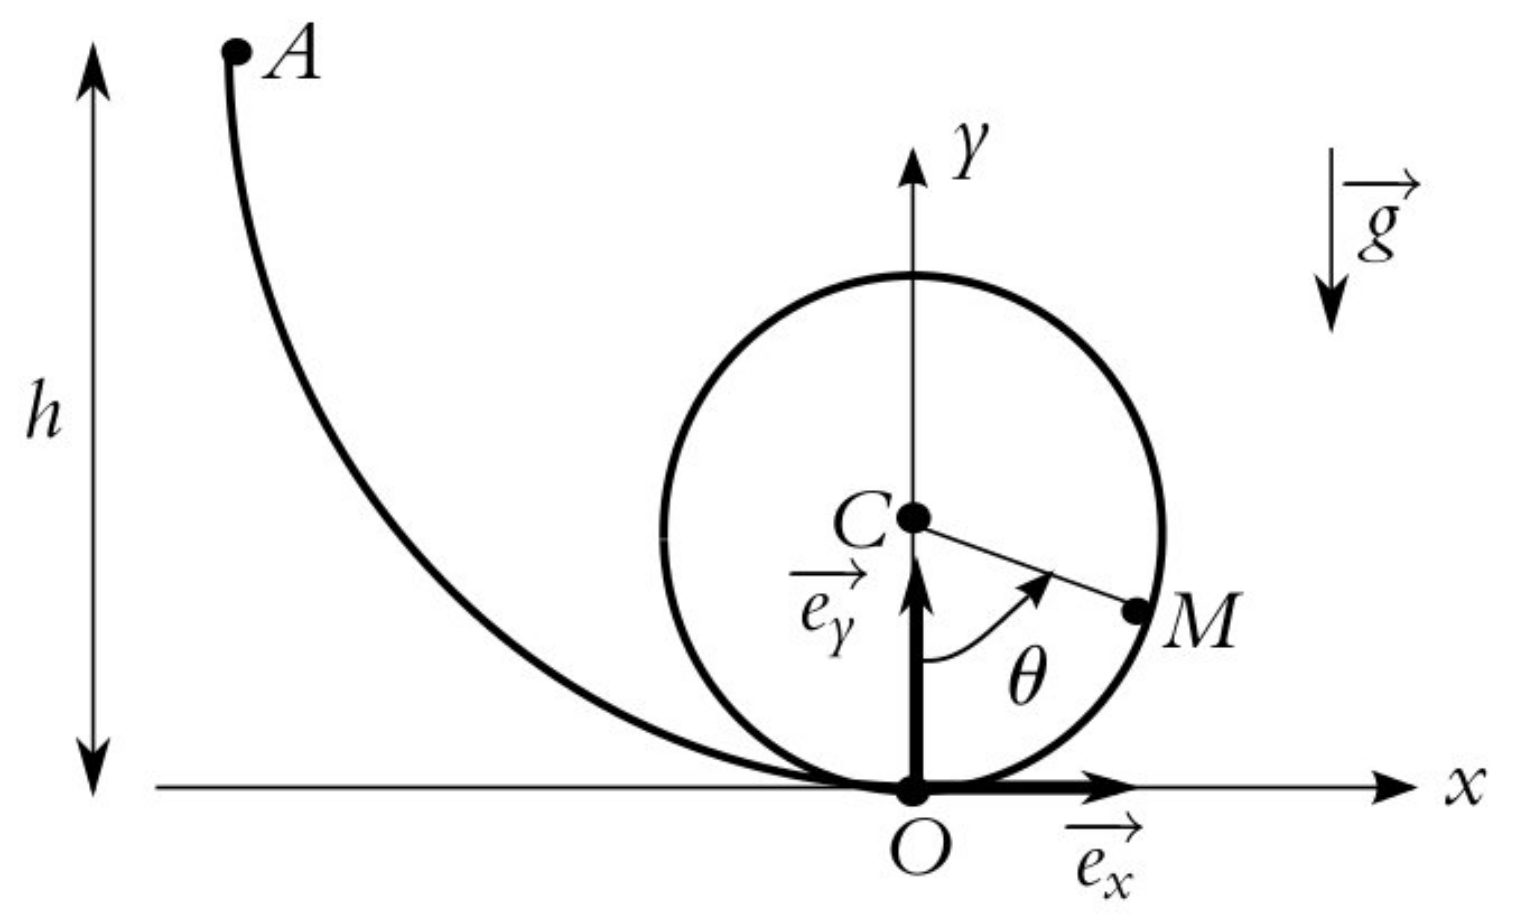
\includegraphics[width=\linewidth]{bille_tonneau-plain}
		\end{center}
	\end{minipage}
}

\QR{%
	Exprimer la norme $v_\Or$ de la vitesse en O, puis $v_\Mr$ en un point
	M quelconque du tonneau repéré par l'angle $\tt$, en fonction de $g$,
	$h$, $a$ et $\tt$. Donner la relation entre $v_\Mr$ et $\tp$.
}{%
	\begin{minipage}[t]{0.65\linewidth}
		\begin{itemize}[label=$\diamond$, leftmargin=10pt]
			\bitem{Système~:} \{balle\}
			\bitem{Référentiel~:} $\Rc\ind{sol}$, supposé galiléen
			\bitem{Repère~:} cartésien pour la chute sur la rampe, avec $\uz$
			vertical ascendant, et $({\rm C}, \ur, \ut)$ quand la balle est
			dans le tonneau~; voir schéma
			\bitem{Repérage~:} dans le tonneau,
			\begin{align*}
				\vv{\rm CM} & = R\ur                \\
				\vf_{\Mr}   & = R\tp\ut             \\
				\af_{\Mr}   & = R\tpp\ut -R\tp^2\ur
			\end{align*}
		\end{itemize}
	\end{minipage}
	\hfill
	\begin{minipage}[t]{0.30\linewidth}
		~
		\begin{center}
			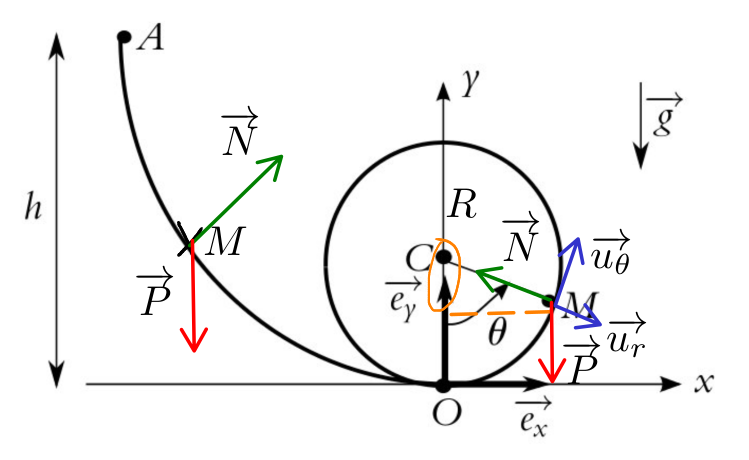
\includegraphics[width=\linewidth]{tonneau_corr}
			\captionsetup{justification=centering}
			\captionof{figure}{Schéma de la situation}
			\label{fig:tonneau_corr}
		\end{center}
	\end{minipage}
	\begin{itemize}[label=$\diamond$, leftmargin=10pt]
		\bitem{BDF~:} dans le tonneau,
		\[
			\begin{array}{ll}
				\textbf{Poids}    & \Pf = mg(\cos\tt\ur-\sin\tt\ut) \\
				\textbf{Réaction} & \Nf = -N\ur
			\end{array}
		\]
		\bitem{BDW~:}
		\begin{align*}
			W_{\rm AM}(\Nf) & = 0 \quad (\Nf\perp\dd\OM) \\
			\Pf             & = \text{conservatif}
		\end{align*}
		Le système est donc \textbf{conservatif}. On peut appliquer le
		TEM~:
		\bitem{En A~:} $v_\Ar = 0$, $z_\Ar = h$
		\bitem{En O~:} $v_\Or = v_\Or$, $\boxed{z_\Or = 0} \Leftarrow$ référence
		\textbf{pour toute l'étude}
		\bitem{En M~:} $z(\tt) = R(1-\cos\tt)$
		\bitem{TEM~:}
		\begin{align*}
			\D_{\rm AO}\Ec_m & = 0
			\\\Lra
			\cancel{m}gh     & = \frac{1}{2}\cancel{m}v_\Or{}^2
			\\\Lra
			\Aboxed{v_\Or    & = \sqrt{2gh}}
			\qed
			\shortintertext{Puis}
			\D_{\rm OM}\Ec_m & = 0
			\\\Lra
			\xoverbracket{\frac{1}{2}\cancel{m}v_\Mr{}^2}^{\Ec_c(\Mr)} +
			\xoverbracket{\cancel{m}gR(1-\cos\tt)}^{\Ec_{p,p}(\Mr)}
			                 & =
			\xoverbracket{\frac{1}{2}\cancel{m}v_\Or{}^2}^{\Ec_c(\Or)} +
			\xoverbracket{\xunderbracket{mgz_\Or}_{=0}}^{\Ec_{p,p}(\Or)}
			\\\Lra
			v_\Mr            & = \sqrt{v_\Or{}^2 + 2gR(\cos\tt-1)}
			\\\Lra
			\Aboxed{v_\Mr    & = \sqrt{2g}\sqrt{h + R(\cos\tt-1)}} = R\tp
			\qed
		\end{align*}
	\end{itemize}
}
\QR{%
	Déterminer la réaction du tonneau en un point du cercle en fonction de
	$g$, $h$, $a$ et $\tt$.
}{%
	On sort de l'analyse énergétique, puisqu'on veut une valeur de force
	\textbf{en un point} du mouvement. On applique donc le \textbf{PFD}~:
	\begin{align*}
		m\af & = \Pf + \Nf
		\\\Lra
		\left\{
		\begin{aligned}
			-mR\tp^2 & = mg\cos\tt-N \\
			mR\tpp   & = -mg\sin\tt
		\end{aligned}
		\right.
		     & \Ra
		N = mg\cos\tt + mR\tp^2
	\end{align*}
	Or, $v_\Mr = R\tp \Lra v_\Mr{}^2 = R^2\tp^2 \Lra R\tp^2 = v_\Mr{}^2/R$
	donc
	\begin{align*}
		N         & = m\left(g\cos\tt + \frac{2g}{R}\left(h+R(\cos\tt-1)\right)\right)
		\\\Lra
		N         & = m\left(g\cos\tt + 2g\cos\tt -2g + 2g \frac{h}{R}\right)
		\\\Lra
		\Aboxed{N & = mg\left(3\cos\tt - 2 + 2 \frac{h}{R}\right)}
		\qed
	\end{align*}
}
\QR{%
	Déterminer la hauteur minimale $h_{\min}$ pour que la bille fasse le
	tour complet du tonneau sans tomber.
}{%
	La condition de contact entre deux solides est que la réaction normale
	ne soit pas nulle. Autrement dit, si la réaction normale est nulle, il
	n'y a plus contact~: on cherche donc ici à voir si $N > 0$ à chaque
	instant. On pourrait tracer la fonction $N(\tt)$, mais on remarque
	facilement que l'endroit où $N$ est la plus susceptible de s'annuler est
	quand $\tt = \pi$, quand la belle est «~la tête à l'envers~». On résout
	donc
	\begin{align*}
		N(\pi)                                    & > 0
		\\\Lra
		\cancel{mg}\left(-3-2+2\frac{g}{R}\right) & > 0
		\\\Lra
		2\frac{h}{R}                              & > 5
		\\\Lra
		\Aboxed{h                                 & > \frac{5}{2}R} = h_{\min}
		\qed
	\end{align*}
}

\end{document}
